% Every number on these slides is produced by the scripts in figures/<dataset>/
% and recorded in figures/<dataset>/numbers_*.txt; quote from those files only.

\section{Why reduce the dimension?}

\begin{frame}{From selecting features to building them}
    \begin{itemize}
        \item Lecture 11: with many features, nearby observations stop existing, distances concentrate and noise features swamp the signal
        \item Selecting a subset of features helps, but it throws features away, even when several of them carry the same information
        \item Idea of this lecture: replace the $p$ original features by $k \ll p$ new ones that keep most of the information
        \item Reasons to do it
            \begin{itemize}
                \item visualization: plot data with many features in two dimensions
                \item compression and noise removal
                \item fewer and uncorrelated inputs for a regression or a classifier
                \item speed: distances and model fits in $k$ dimensions instead of $p$
            \end{itemize}
    \end{itemize}
\end{frame}

\begin{frame}{Correlated features carry the same information twice}
    \begin{columns}[T]
        \begin{column}{0.54\textwidth}
            \begin{itemize}
                \item In the Credit data, Limit and Rating have correlation 0.997 (lecture 11)
                \item The standardized points form a long, thin ellipse
                \item One axis along it, $0.707 \cdot \text{Limit} + 0.707 \cdot \text{Rating}$, carries 99.8\% of the variance
                \item The axis across the ellipse adds almost nothing
            \end{itemize}
        \end{column}
        \begin{column}{0.44\textwidth}
            \centering
            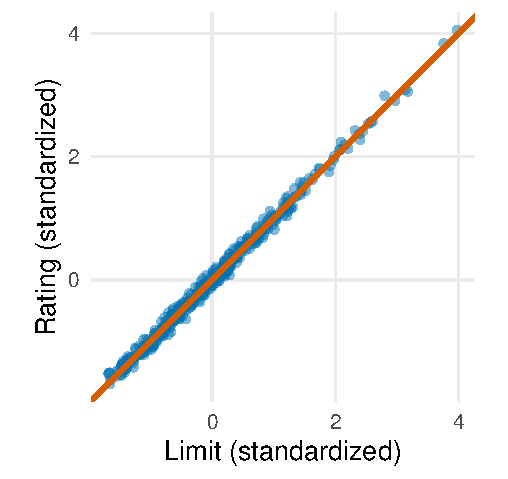
\includegraphics[width=\textwidth, height=0.65\textheight, keepaspectratio]{figures/credit/fig_two_features_axis.pdf}

            {\scriptsize Credit: standardized Limit and Rating, with the long axis}
        \end{column}
    \end{columns}
\end{frame}

\begin{frame}{Selection vs. extraction, and the plan}
    \begin{itemize}
        \item Selection keeps a subset of the original features: interpretable, but the dropped features are gone
        \item Extraction builds a few new features, each a linear combination of all the original ones: harder to interpret, but it keeps the shared information of correlated features
        \item Today's tool is principal component analysis (PCA), which builds the combinations in order of how much variance they capture
        \item Plan
            \begin{enumerate}
                \item the singular value decomposition (SVD) in brief, because PCA is computed from it
                \item PCA: definition, interpretation, how many components
                \item using PCA: regression, visualization, clustering, denoising
            \end{enumerate}
    \end{itemize}
\end{frame}


\section{The SVD in brief}

\begin{frame}{The data matrix}
    \begin{itemize}
        \item Collect the data in an $n \times p$ matrix $X$: one row per observation, one column per feature
        \item Center every column by subtracting its mean; if the features have different units, also divide by the SD (lecture 11)
        \item From now on, $X$ is this centered (and, where needed, standardized) matrix
        \item Examples: USArrests has $n = 50$ and $p = 4$; the digits have $n = 3{,}823$ images and $p = 64$ pixels; NCI60 has $n = 64$ and $p = 6{,}830$ genes
    \end{itemize}
\end{frame}

\begin{frame}{The singular value decomposition}
    \begin{columns}[T]
        \begin{column}{0.5\textwidth}
            \begin{itemize}
                \item Every matrix can be written as
                    \[
                        X = U \Sigma V^\top
                    \]
                \item $U$ and $V$ have orthonormal columns, and $\Sigma$ is diagonal with $\sigma_1 \ge \sigma_2 \ge \dots \ge 0$, the singular values
                \item In PCA, the columns of $V$ will be the directions (loadings), $U \Sigma$ the new feature values (scores), and $\sigma_j^2$ the variance along direction $j$
            \end{itemize}
        \end{column}
        \begin{column}{0.48\textwidth}
            \centering
            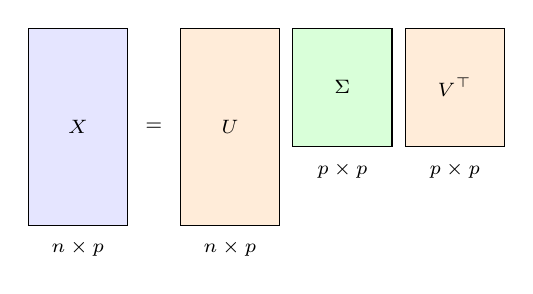
\begin{tikzpicture}[x=0.42cm, y=0.5cm, font=\scriptsize]
                \draw[fill=blue!10] (0, 0) rectangle (3, 5);
                \node at (1.5, 2.5) {$X$};
                \node at (1.5, -0.6) {$n \times p$};
                \node at (3.8, 2.5) {$=$};
                \draw[fill=orange!15] (4.6, 0) rectangle (7.6, 5);
                \node at (6.1, 2.5) {$U$};
                \node at (6.1, -0.6) {$n \times p$};
                \draw[fill=green!15] (8.0, 2.0) rectangle (11.0, 5);
                \node at (9.5, 3.5) {$\Sigma$};
                \node at (9.5, 1.4) {$p \times p$};
                \draw[fill=orange!15] (11.4, 2.0) rectangle (14.4, 5);
                \node at (12.9, 3.5) {$V^\top$};
                \node at (12.9, 1.4) {$p \times p$};
            \end{tikzpicture}

            \svspace{0.3em}
            {\scriptsize Shown for $n > p$; $\Sigma$ is zero off the diagonal}
        \end{column}
    \end{columns}
\end{frame}

\begin{frame}{The best low-rank approximation}
    \begin{itemize}
        \item Keep only the first $k$ singular values: $X_k = \sum_{j=1}^{k} \sigma_j \mathbf{u}_j \mathbf{v}_j^\top$
        \item Eckart-Young: among all matrices of rank $k$, $X_k$ is the closest to $X$ in squared error, and the error is
            \[
                \sum_{i,j} (x_{ij} - x^{(k)}_{ij})^2 = \sum_{j > k} \sigma_j^2
            \]
        \item We state this without proof; it is the one fact used later, for reconstruction and denoising
        \item The SVD also appears in image compression, recommender systems (latent factors), text analysis (latent semantic analysis) and least squares via the pseudoinverse (lecture 3)
    \end{itemize}
\end{frame}


\section{Principal component analysis}

\begin{frame}{The goal}
    \begin{itemize}
        \item Find the direction in feature space along which the data vary the most; then the direction of most variation among those orthogonal to the first; and so on
        \item These directions are the principal components, and the data expressed along them are the scores
        \item Behind this: variance is treated as information. A direction in which all observations look alike tells us little; a direction in which they differ tells us a lot
        \item We will see that this is an assumption, and that it can fail
    \end{itemize}
\end{frame}

\begin{frame}{The first principal component}
    \begin{columns}[T]
        \begin{column}{0.56\textwidth}
            \begin{itemize}
                \item The first loading vector $\mathbf{v}_1$ (length 1) maximizes the variance of the scores:
                    \[
                        \mathbf{v}_1 = \arg\max_{\lVert \mathbf{v} \rVert = 1} \operatorname{Var}(X \mathbf{v})
                    \]
                \item The same line minimizes the squared distances to the points: variance along the line plus squared distance to it is the total
                \item Simulated, 40 points: $4.58 + 0.231 = 4.814$
            \end{itemize}
        \end{column}
        \begin{column}{0.42\textwidth}
            \centering
            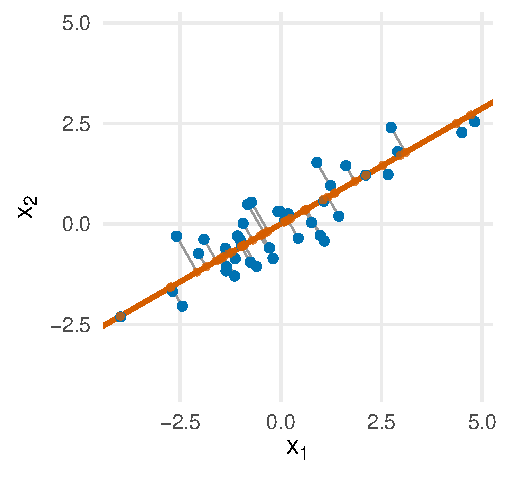
\includegraphics[width=\textwidth, height=0.6\textheight, keepaspectratio]{figures/simulated/fig_pc1_line.pdf}

            {\scriptsize Points, first component and projections}
        \end{column}
    \end{columns}
\end{frame}

\begin{frame}{Further components}
    \begin{itemize}
        \item The second component $\mathbf{v}_2$ maximizes the variance among directions orthogonal to $\mathbf{v}_1$, the third among those orthogonal to both, and so on
        \item The scores of different components are uncorrelated
        \item At most $\min(n - 1, p)$ components have nonzero variance: USArrests has 4, NCI60 has 63 (64 samples, 6{,}830 genes), and the digits have 62, because two of the 64 pixels never change
        \item Together the components are a rotation of the original axes: nothing is lost until we drop some of them
    \end{itemize}
\end{frame}

\begin{frame}{PCA through the SVD}
    \centering
    \footnotesize
    \begin{tabular}{@{}l l l@{}}
        \toprule
        SVD object & PCA name & Meaning \\
        \midrule
        Columns of $V$ & loadings & weight of each feature in a component \\
        $X V = U \Sigma$ & scores & the new feature values \\
        $\sigma_j^2 / (n - 1)$ & variance of component $j$ & eigenvalue of $\frac{1}{n-1} X^\top X$ \\
        \bottomrule
    \end{tabular}

    \svspace{0.8em}
    \raggedright
    \begin{itemize}
        \item USArrests (standardized): singular values 11.02, 6.96, 4.18 and 2.92; $\sigma_j^2 / 49$ gives the variances 2.48, 0.99, 0.36 and 0.17, identical to \texttt{prcomp}
        \item Loadings from the SVD and from \texttt{prcomp} agree exactly; the scores are uncorrelated (largest correlation $4.5 \times 10^{-16}$)
        \item Software uses the SVD rather than the eigenvalues because it is numerically more stable
    \end{itemize}
\end{frame}

\begin{frame}{Example: PCA on USArrests}
    \centering
    \footnotesize
    \begin{tabular}{@{}l r r r r@{}}
        \toprule
        & PC1 & PC2 & PC3 & PC4 \\
        \midrule
        Murder & 0.536 & $-0.418$ & 0.341 & 0.649 \\
        Assault & 0.583 & $-0.188$ & 0.268 & $-0.743$ \\
        UrbanPop & 0.278 & 0.873 & 0.378 & 0.134 \\
        Rape & 0.543 & 0.167 & $-0.818$ & 0.089 \\
        \bottomrule
    \end{tabular}

    \svspace{0.8em}
    \raggedright
    \begin{itemize}
        \item PC1 weighs the three crime rates about equally and UrbanPop less: an overall level of violent crime
        \item PC2 is dominated by UrbanPop, with the opposite sign on Murder and Assault: the degree of urbanization
        \item The signs of a whole component are arbitrary; here the loadings of each component are oriented to sum to a positive number
    \end{itemize}
\end{frame}

\begin{frame}{Scores and the biplot}
    \begin{columns}[T]
        \begin{column}{0.38\textwidth}
            \begin{itemize}
                \item Each state is a point at its scores on PC1 and PC2; arrows show the loadings
                \item Florida, Nevada and California are high on PC1; North Dakota and Vermont are low
                \item Only two components are shown, so distances in the plot are approximate
            \end{itemize}
        \end{column}
        \begin{column}{0.6\textwidth}
            \centering
            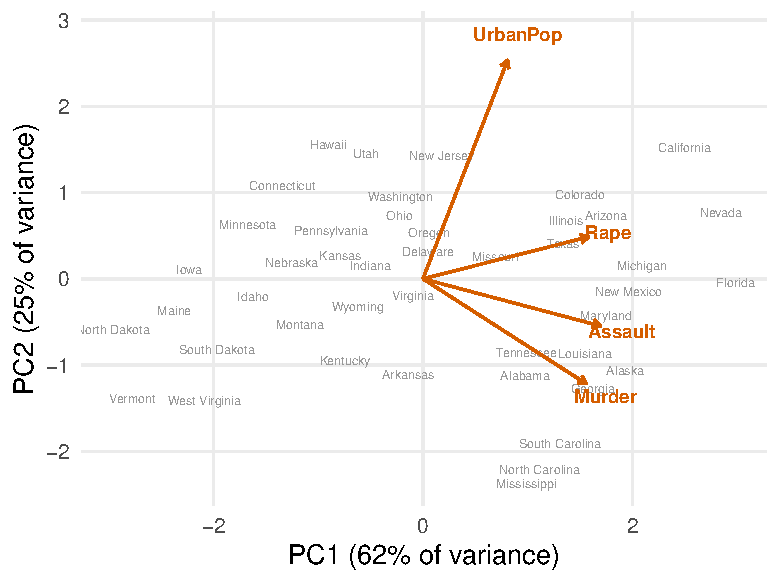
\includegraphics[width=\textwidth, height=0.8\textheight, keepaspectratio]{figures/usarrests/fig_usarrests_biplot.pdf}
        \end{column}
    \end{columns}
\end{frame}

\begin{frame}{Scaling matters, again}
    \begin{columns}[T]
        \begin{column}{0.56\textwidth}
            \begin{itemize}
                \item PCA looks for variance, so variables with a large SD dominate (lecture 11)
                \item Raw USArrests: PC1 explains 96.6\% and is almost only Assault (loading 0.995)
                \item Standardized: loadings 0.54, 0.58 and 0.54 on the three crime rates
                \item Standardize unless all features share one meaningful unit (the digit pixels are only centered)
            \end{itemize}
        \end{column}
        \begin{column}{0.42\textwidth}
            \centering
            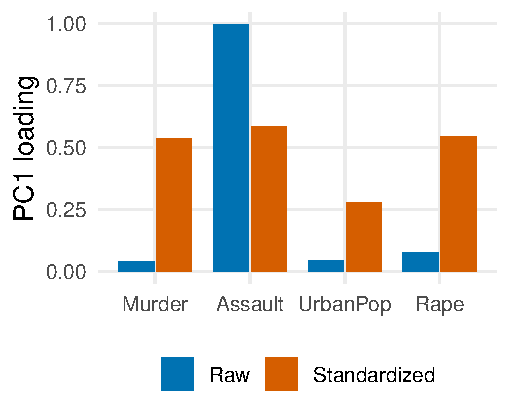
\includegraphics[width=\textwidth, height=0.55\textheight, keepaspectratio]{figures/usarrests/fig_pca_scaling.pdf}

            {\scriptsize PC1 loadings, raw and standardized}
        \end{column}
    \end{columns}
\end{frame}

\begin{frame}{Proportion of variance explained}
    \begin{itemize}
        \item Component $j$ explains
            \[
                \text{PVE}_j = \frac{\sigma_j^2}{\sum_{i} \sigma_i^2}
            \]
            of the total variance; the PVEs add up to 1
        \item USArrests: 62.0\%, 24.7\%, 8.9\% and 4.3\%; the first two together 86.8\%
        \item Digits: 14.9\%, 13.4\% and 11.7\% for the first three; the first 10 components 74.1\%, the first 30 95.8\%
        \item NCI60: only 11.4\% and 6.8\% for the first two, and 44 components for 90\%
        \item PVE tells how much of the spread a summary keeps, not how useful it is for prediction
    \end{itemize}
\end{frame}

\begin{frame}{How many components?}
    \begin{itemize}
        \item Scree plot: plot the variance of each component and look for an elbow where the curve flattens
        \item Cumulative variance: keep enough components to reach a threshold such as 90\%
        \item Kaiser rule (standardized data): keep components whose variance exceeds 1, the variance of a single standardized feature
        \item Cross-validation: choose the number that gives the best error in the task that follows (regression, classification), the most direct answer
        \item There is no single right answer: the rules are guides, and the choice depends on what the components are for
    \end{itemize}
\end{frame}

\begin{frame}{Scree plots}
    \begin{columns}[T]
        \begin{column}{0.5\textwidth}
            \centering
            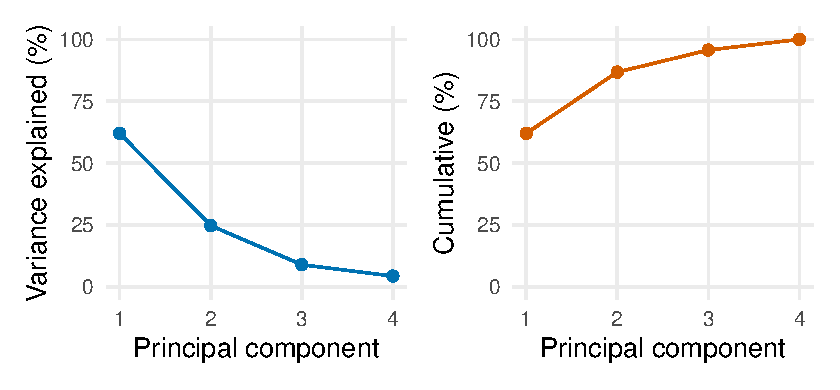
\includegraphics[width=\textwidth, height=0.38\textheight, keepaspectratio]{figures/usarrests/fig_scree_usarrests.pdf}

            {\scriptsize USArrests: the elbow is at PC2}

            \svspace{0.3em}
            \begin{itemize}
                \item Kaiser rule: keep PC1 only (PC2 has variance 0.99)
                \item But PC2 explains 24.7\% and means urbanization, so we keep two
            \end{itemize}
        \end{column}
        \begin{column}{0.48\textwidth}
            \centering
            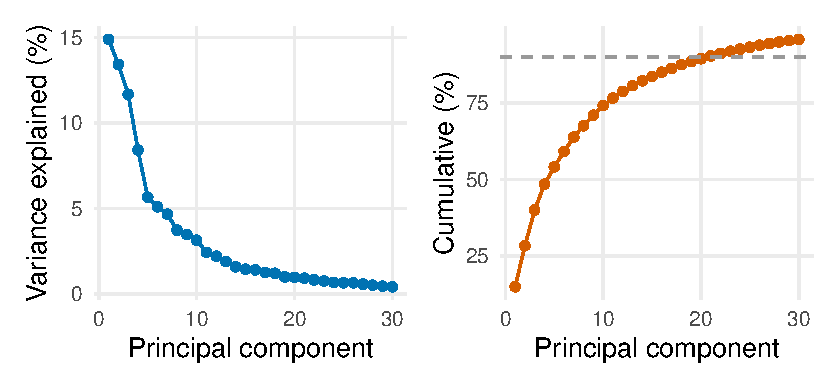
\includegraphics[width=\textwidth, height=0.38\textheight, keepaspectratio]{figures/digits/fig_digits_scree.pdf}

            {\scriptsize Digits: no sharp elbow; dashed line at 90\%}

            \svspace{0.3em}
            \begin{itemize}
                \item 21 components reach 90\%, 30 reach 95.8\%
                \item A threshold or cross-validation has to decide
            \end{itemize}
        \end{column}
    \end{columns}
\end{frame}

\begin{frame}{Reconstruction: what is lost?}
    \begin{columns}[T]
        \begin{column}{0.55\textwidth}
            \begin{itemize}
                \item Project on the first $k$ components and back: $\hat{X}_k = X V_k V_k^\top$ (add the means back)
                \item This is the rank-$k$ approximation, so the squared error is the sum of the dropped $\sigma_j^2$
                \item USArrests, 2 components: error 25.97 $= \sigma_3^2 + \sigma_4^2$
                \item Digits, mean squared error per pixel: 13.48 with 2 components, 4.86 with 10, 0.79 with 30
            \end{itemize}
        \end{column}
        \begin{column}{0.43\textwidth}
            \centering
            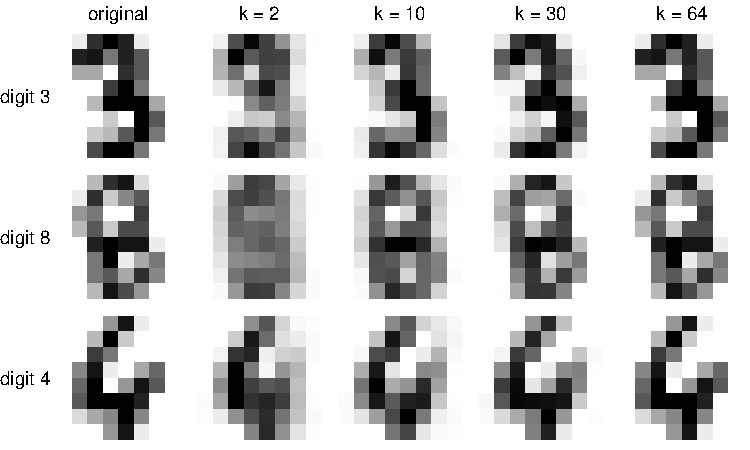
\includegraphics[width=\textwidth, height=0.55\textheight, keepaspectratio]{figures/digits/fig_digits_reconstruction.pdf}

            {\scriptsize Three digits rebuilt from $k$ components}
        \end{column}
    \end{columns}
\end{frame}

\begin{frame}{Variance is not the same as relevance}
    \begin{columns}[T]
        \begin{column}{0.56\textwidth}
            \begin{itemize}
                \item PCA never looks at class labels
                \item Simulated: $x_1$ has a large spread and no class information; the classes differ along $x_2$, which has a small spread
                \item PC1 is $x_1$ (loading 0.999) and explains 89\% of the variance, but a threshold on PC1 gets 56\% right; on PC2, 95.5\%
                \item Dropping low-variance components can drop the useful ones
            \end{itemize}
        \end{column}
        \begin{column}{0.42\textwidth}
            \centering
            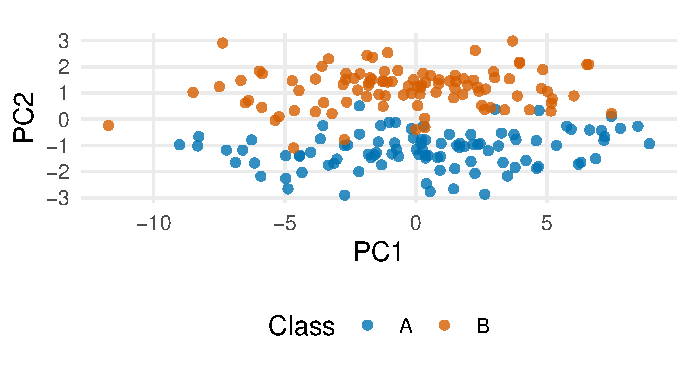
\includegraphics[width=\textwidth, height=0.45\textheight, keepaspectratio]{figures/simulated/fig_pca_variance_not_relevance.pdf}

            {\scriptsize Scores on PC1 and PC2, by class}
        \end{column}
    \end{columns}
\end{frame}

\begin{frame}{Properties and limits}
    \begin{itemize}
        \item Components are linear combinations of the features and are uncorrelated with each other
        \item PCA only finds linear structure (a later slide shows a curved example)
        \item Outliers pull the components toward themselves, because the criterion is squared distance
        \item Signs are arbitrary: flipping a loading vector and its scores changes nothing, so compare components only up to sign
        \item Components with nearly equal variance are not well defined: a small change in the data can rotate them within their plane
        \item Components are harder to interpret than the original features; reading the loadings is part of the analysis
    \end{itemize}
\end{frame}

\begin{frame}{PCA in practice}
    \begin{itemize}
        \item Order of steps: split the data, standardize (where needed) and fit PCA on the training data only, then apply the same transformation to the test data
        \item As with scalers (lecture 11), fitting on all the data lets the test data influence the transformation, which is leakage
        \item Inside cross-validation, put the scaler and PCA in a pipeline together with the model, so both are refitted in every fold
        \item In scikit-learn, \texttt{PCA(n\_components=k)} fixes the number of components; \texttt{PCA(n\_components=0.9)} keeps as many as are needed to explain 90\% of the variance
        \item \texttt{explained\_variance\_ratio\_} gives the PVEs, \texttt{components\_} the loadings, and \texttt{inverse\_transform} the reconstruction
    \end{itemize}
\end{frame}


\section{Feature extraction and visualization}

\begin{frame}{Scores as inputs to a model}
    \begin{columns}[T]
        \begin{column}{0.55\textwidth}
            \begin{itemize}
                \item Use the first $k$ scores instead of the $p$ features as inputs
                \item Fewer, uncorrelated inputs help linear models; $k$-NN computes distances in $k$ dimensions
                \item Digits, 5-NN, PCA fitted on the 3{,}823 training images, tested on 1{,}797 others
                \item Accuracy 0.563 with 2 components, 0.904 with 5, 0.953 with 10, 0.978 with 20: the same as all 64 pixels
            \end{itemize}
        \end{column}
        \begin{column}{0.43\textwidth}
            \centering
            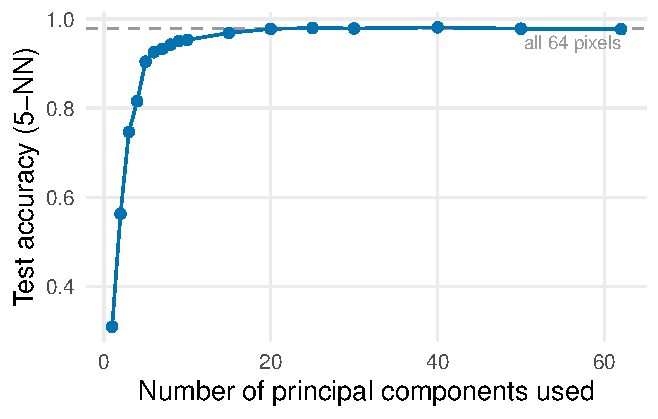
\includegraphics[width=\textwidth, height=0.55\textheight, keepaspectratio]{figures/digits/fig_digits_knn_pca.pdf}

            {\scriptsize Test accuracy of 5-NN on the first $k$ components}
        \end{column}
    \end{columns}
\end{frame}

\begin{frame}{Principal components regression}
    \begin{columns}[T]
        \begin{column}{0.58\textwidth}
            \begin{itemize}
                \item Principal components regression (PCR): regress on the first $k$ scores, choose $k$ by cross-validation
                \item It handles multicollinearity (lecture 4): Hitters has 12 pairs of predictors with $|r| > 0.9$
                \item 10-fold CV RMSE: 452 with no predictor, 351.9 with 1 component, 339.2 at best (18), 339.6 with all 19 (OLS), 343.6 with 6
                \item Caveat: the components are built without the response
            \end{itemize}
        \end{column}
        \begin{column}{0.4\textwidth}
            \centering
            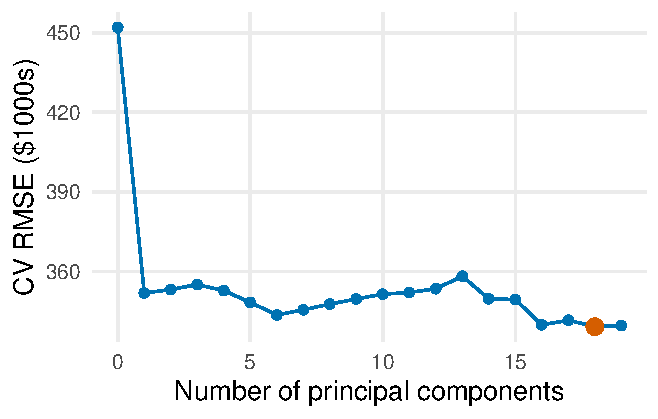
\includegraphics[width=\textwidth, height=0.5\textheight, keepaspectratio]{figures/hitters/fig_pcr_cv.pdf}

            {\scriptsize Hitters: CV error of PCR, in \$1000s}
        \end{column}
    \end{columns}
\end{frame}

\begin{frame}{Selection, extraction, and PCR compared}
    \centering
    \footnotesize
    \begin{tabular}{@{}l l c l@{}}
        \toprule
        & Features used & Uses response & Interpretation \\
        \midrule
        Lasso & subset of the originals & yes & original features \\
        PCA & combinations of all & no & loadings \\
        PCR & first $k$ PCA scores & only for $k$ & loadings \\
        PLS & combinations built for the response & yes & loadings \\
        \bottomrule
    \end{tabular}

    \svspace{0.8em}
    \raggedright
    \begin{itemize}
        \item PLS (partial least squares) builds components from the covariance of the features with the response, so a predictive low-variance direction is not dropped
        \item Ridge keeps all features and shrinks their coefficients, most along the low-variance principal components
    \end{itemize}
\end{frame}

\begin{frame}{Comparison on Hitters}
    \begin{columns}[T]
        \begin{column}{0.54\textwidth}
            \begin{itemize}
                \item 10-fold CV RMSE (\$1000s): PCR 339.2, PLS 338.3, ridge 334.1, lasso 332.4 (13 of 19 predictors)
                \item All within about 3\%: PCR is not the winner here
                \item With one component PLS reaches 349.2 and PCR 351.9, because the PLS component uses Salary
                \item Differences of a few units are within the noise of the folds
            \end{itemize}
        \end{column}
        \begin{column}{0.44\textwidth}
            \centering
            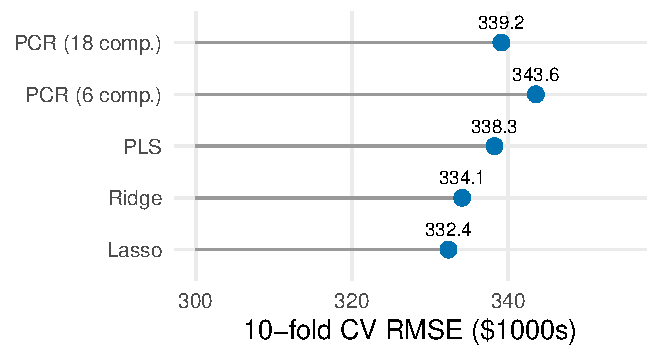
\includegraphics[width=\textwidth, height=0.55\textheight, keepaspectratio]{figures/hitters/fig_pcr_vs_others.pdf}

            {\scriptsize Hitters: 10-fold CV RMSE}
        \end{column}
    \end{columns}
\end{frame}

\begin{frame}{Visualizing high-dimensional data}
    \begin{columns}[T]
        \begin{column}{0.46\textwidth}
            \begin{itemize}
                \item Plot the first two scores, colored by a variable that PCA did not use
                \item Digits: PC1 and PC2 hold only 28.3\%, yet 0, 6, 7 and 4 sit in different corners, while 5 and 8 overlap
                \item Between-digit share of variance in this plane: 0.741, against 0.415 for a typical pair of pixels
                \item Report the PVE on the axes
            \end{itemize}
        \end{column}
        \begin{column}{0.52\textwidth}
            \centering
            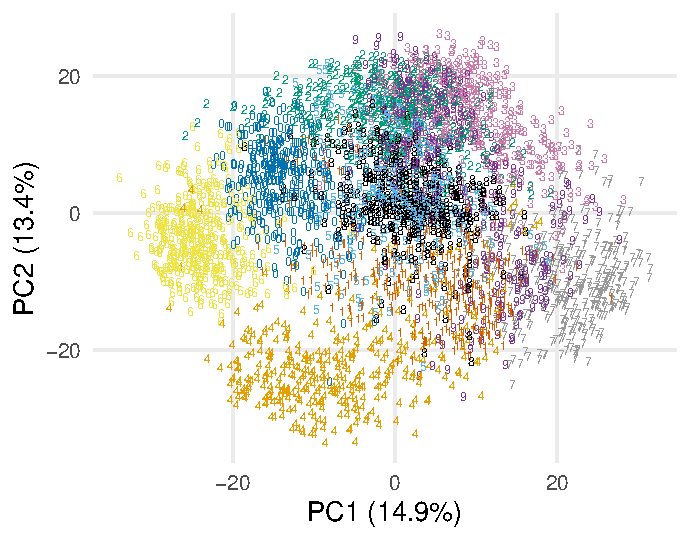
\includegraphics[width=\textwidth, height=0.75\textheight, keepaspectratio]{figures/digits/fig_digits_pca.pdf}
        \end{column}
    \end{columns}
\end{frame}

\begin{frame}{Example: NCI60 gene expression}
    \begin{columns}[T]
        \begin{column}{0.4\textwidth}
            \begin{itemize}
                \item 64 cell lines, 6{,}830 genes, 14 cancer types (lecture 10)
                \item With $n < p$ there are at most 63 components; the first five explain 31.8\%
                \item In the PC1-PC2 plane 72.7\% of the variance is between cancer types; for random pairs of genes the median is 32.2\%
            \end{itemize}
        \end{column}
        \begin{column}{0.58\textwidth}
            \centering
            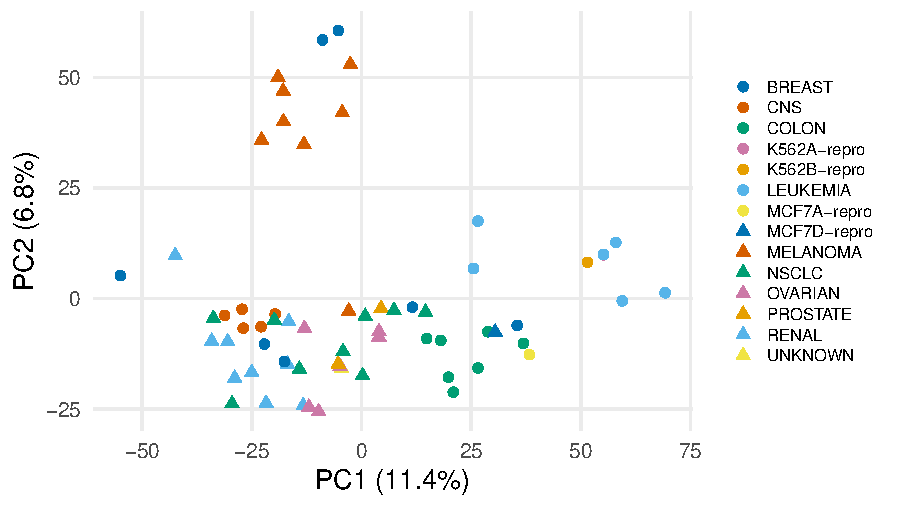
\includegraphics[width=\textwidth, height=0.75\textheight, keepaspectratio]{figures/nci60/fig_nci60_pca.pdf}
        \end{column}
    \end{columns}
\end{frame}

\begin{frame}{Clustering in the space of the components}
    \begin{columns}[T]
        \begin{column}{0.54\textwidth}
            \begin{itemize}
                \item Cluster the first $k$ scores instead of 6{,}830 genes: cheaper, and the small, mostly noisy components are ignored
                \item Complete linkage; agreement with the 14 cancer types by the adjusted Rand index (1 perfect, 0 chance)
                \item 14 clusters: 0.265 with all genes, 0.388 with 5 components; 4 clusters: 0.127 and 0.135
                \item At least as good, but not magic
            \end{itemize}
        \end{column}
        \begin{column}{0.44\textwidth}
            \centering
            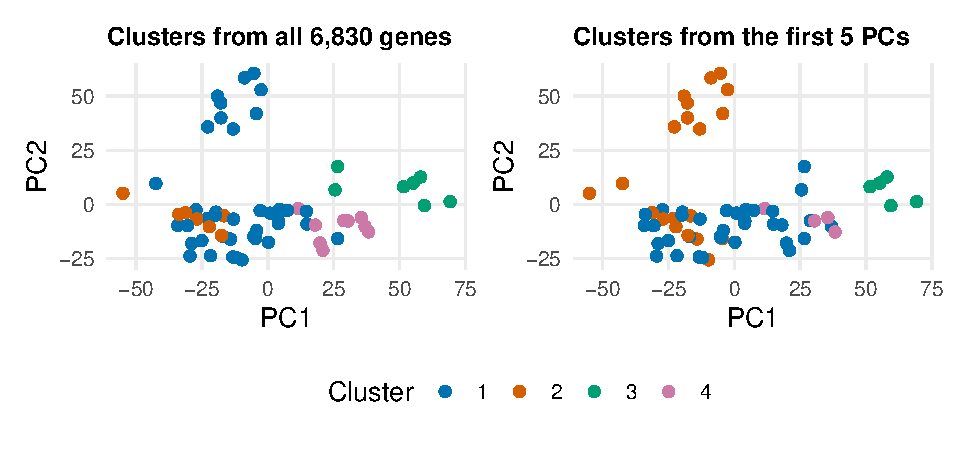
\includegraphics[width=\textwidth, height=0.45\textheight, keepaspectratio]{figures/nci60/fig_nci60_cluster_pca.pdf}

            {\scriptsize Four clusters, from all genes and from 5 components}
        \end{column}
    \end{columns}
\end{frame}

\begin{frame}{Denoising}
    \begin{columns}[T]
        \begin{column}{0.56\textwidth}
            \begin{itemize}
                \item The signal sits in a few high-variance directions, the noise is spread over all of them
                \item Keep the top components and reconstruct
                \item Digits with noise (SD 4 on a 0 to 16 scale), PCA fitted on noisy images; error against the clean ones: 15.9 noisy, 7.5 with 10 components, 7.2 with 20, 10.4 with 40
                \item Best $k = 16$ (7.0): too many components put the noise back
            \end{itemize}
        \end{column}
        \begin{column}{0.42\textwidth}
            \centering
            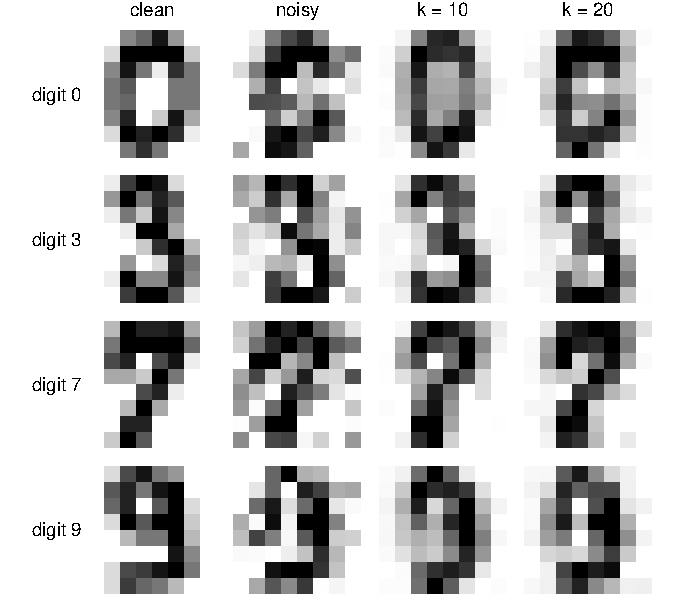
\includegraphics[width=\textwidth, height=0.8\textheight, keepaspectratio]{figures/digits/fig_digits_denoise.pdf}
        \end{column}
    \end{columns}
\end{frame}

\begin{frame}{Beyond linear PCA}
    \begin{columns}[T]
        \begin{column}{0.38\textwidth}
            \begin{itemize}
                \item A Swiss roll is a flat sheet rolled up in 3-D: the data are two-dimensional but curved
                \item PCA flattens the roll and puts far-apart points together: it keeps 17\% of each point's 10 nearest neighbors on the sheet
                \item t-SNE keeps 61\%
            \end{itemize}
        \end{column}
        \begin{column}{0.6\textwidth}
            \centering
            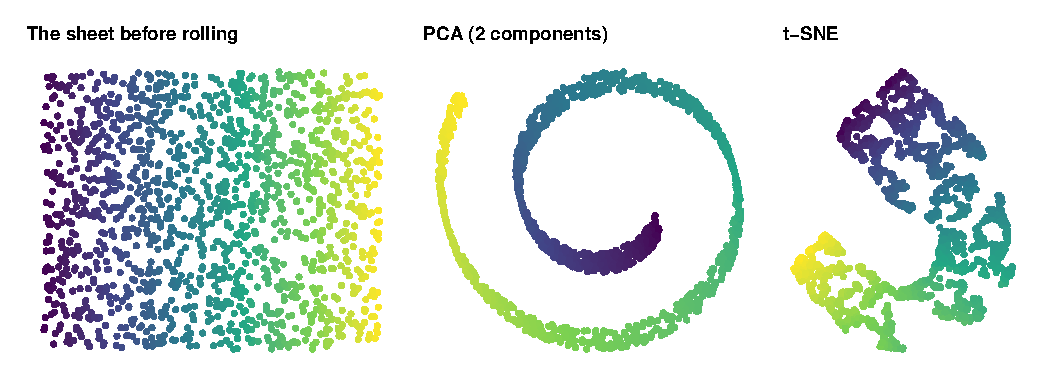
\includegraphics[width=\textwidth, height=0.45\textheight, keepaspectratio]{figures/simulated/fig_swiss_roll.pdf}

            {\scriptsize Colored by position along the roll}
        \end{column}
    \end{columns}
\end{frame}

\begin{frame}{Nonlinear alternatives}
    \begin{itemize}
        \item Kernel PCA: PCA after an implicit nonlinear map of the features
        \item t-SNE and UMAP: embeddings that keep neighborhoods; used for visualization only
            \begin{itemize}
                \item distances between far-apart clusters are not meaningful
                \item the picture depends on hyperparameters, such as the perplexity in t-SNE
            \end{itemize}
        \item Autoencoders: neural networks that compress and reconstruct their input; with linear layers they find the same subspace as PCA (next lecture)
        \item We use PCA first: it is fast, deterministic, has a clear meaning, and gives a baseline
    \end{itemize}
\end{frame}

\begin{frame}{Choosing a method}
    \centering
    \footnotesize
    \begin{tabular}{@{}l l@{}}
        \toprule
        Situation & Start with \\
        \midrule
        Correlated predictors in a regression & PCR or PLS, or ridge and lasso \\
        Visualize high-dimensional data & PCA, then t-SNE or UMAP \\
        Need interpretable features & selection (lecture 11), or inspect the loadings \\
        Noisy features or images & PCA with $k$ chosen by cross-validation \\
        Sparse text data & \texttt{TruncatedSVD} (no centering) \\
        Class labels, want separation & linear discriminant analysis (lecture 6) \\
        \bottomrule
    \end{tabular}

    \svspace{0.8em}
    \raggedright
    \begin{itemize}
        \item In all cases, scale first (where needed), fit on the training data only, and choose $k$ by cross-validation
    \end{itemize}
\end{frame}


\section{Summary}

\begin{frame}{PCA in Python}
    \centering
    \scriptsize
    \begin{tabular}{@{}l l@{}}
        \toprule
        Task & Python (\texttt{sklearn}) \\
        \midrule
        Standardize & \texttt{preprocessing.StandardScaler} \\
        PCA & \texttt{decomposition.PCA(n\_components=k)}, or \texttt{n\_components=0.9} \\
        Loadings, PVEs & \texttt{components\_}, \texttt{explained\_variance\_ratio\_} \\
        Scores, reconstruction & \texttt{transform}, \texttt{inverse\_transform} \\
        Sparse data & \texttt{decomposition.TruncatedSVD} \\
        Pipeline and CV & \texttt{pipeline.make\_pipeline}, \texttt{model\_selection.cross\_val\_score} \\
        PCR (pipeline) & \texttt{make\_pipeline(StandardScaler(), PCA(), LinearRegression())} \\
        PLS & \texttt{cross\_decomposition.PLSRegression} \\
        Nonlinear embeddings & \texttt{manifold.TSNE}, \texttt{decomposition.KernelPCA} \\
        \bottomrule
    \end{tabular}

    \svspace{0.5em}
    Worked examples: the ISLP Python lab, Section 12.5
\end{frame}

\begin{frame}{Summary}
    \begin{itemize}
        \item PCA builds new features, in order of variance, from the SVD of the centered (usually standardized) data
        \item Loadings say what a component means, scores are the new data, PVE says how much is kept; choose $k$ by a scree plot, a variance threshold or cross-validation
        \item Rebuilding from $k$ components is the best rank-$k$ approximation
        \item Use it for visualization, as inputs to regression and clustering, and for denoising, with scaling and PCA fitted on the training data inside the pipeline
        \item Variance is not relevance, and PCA sees only linear structure
        \item Reading: ISLP 6.3 and 12.2; ESL 3.5 and 14.5
        \item Next lecture: neural networks, which learn features; an autoencoder is a nonlinear PCA
    \end{itemize}
\end{frame}
